\chapter{The Deep Learning Algorithm}
\label{chap:Algorithm}



This chapter focuses on discussing the deep learning algorithm that has been implemented and tested throughout the work.
Although we have been using this algorithm with a data quality monitoring goal in mind, it stems from the search for new
physics at LHC. The fact that the algorithm can be employed in both fields clearly shows the sound flexibility of both
the conceptual foundations and the practical implementation. Hence, the first part of this chapter focuses on delivering
a general introduction to the algorithm's statistical background. Then, we share an overview of its actual functioning
and how it can be employed in data quality monitoring.

\section{Conceptual foundations}
% \section{Introduction to Deep Learning techniques in Physics}
% \label{sec:dltphysics}

% The most widely employed approach to detect discrepancies in data falls under the name of anomaly detection. 



% % The most widely employed approach to the problem is to search for events of specific new physics models. In any such
% % model, one can identify a priori the subset of data where large departures from the reference model should be
% % concentrated. In this sense, this is a biased search for anomalies. While this procedure provides a clear physical
% % insight into the new phenomena, scientists have come to realize that employing a model-dependent approach has a critical
% % disadvantage: a statistical test designed to be sensitive to one specific hypothesis is typically insensitive to data
% % departures of a different nature from the one expected. This means that if new physics is present in the data, but not
% % predicted by the specific model that is being tested, it would not be discovered. 

% \subsection{Model-independent approach}

% Many attempts at generalizing traditional model-dependent approach have already been made, developing the so-called
% model-independent search strategies. It is crucial to remark that model-independent hypothesis testing is an ill-defined
% concept in statistics: testing the reference unavoidably requires an alternative hypothesis against which the test is
% performed. In a model-independent approach, the alternative hypothesis is not built from a specific physical model but
% is a flexible one. The alternative hypothesis is thus a model which specifies a flexible expected density distribution
% that can approximate the true underlying data distribution. The algorithm presented in this chapter, proposed in
% \cite{zanetti} and \cite{wulzer}, uses NNs to parametrize the alternative distribution to detect deviations from the
% reference model in experimental datasets with no prior knowledge of the nature of the discrepancies. 


% \subsection{Stsatistical background}
\label{sec:foundations}

The whole construction of the statistical background that underpins the algorithm is accurately discussed in
\textit{Learning New Physics from a Machine (2018)} by R. T. D'Agnolo and A. Wulzer \cite{wulzer}. Thus, we give only a
brief recap on the construction of hypothesis testing with neural networks involved. 

Let us consider then a dataset of repeated measurements
$\mathbfcal{D}=\{x_i\}_{i=1\,\ldots\,\mathcal{N}_{\mathbfcal{D}}}$ of a \textit{d}-dimensional random variable $x$. Let
$n(x\,|\,\mathbfcal{R})$ be its expected differential distribution as predicted by the reference model
$\mathbfcal{R}\,(\,\equiv H_0$, i.e. the null hypothesis): it can be written as 

\begin{equation}
    n(x\,|\,\mathbfcal{R}) = \mathcal{N}(\mathbfcal{R})\,\,p(x\,|\,\mathbfcal{R})
\end{equation}

\noindent where $p(x\,|\,\mathbfcal{R})$ is the probability density function related to the reference hypothesis and
$\mathcal{N}_{\mathbfcal{R}}^{\text{exp}}$ is the total number of expected events to be found in the experimental
dataset according to $\mathbfcal{R}$, given by 

\begin{equation}
    \mathcal{N}(\mathbfcal{R})=\int  n(x\,|\,\mathbfcal{R}) \, \text{d}x
\end{equation}


\noindent If the dataset $\mathbfcal{D}$ follows the reference hypothesis, then the total number of events
observed in $\mathbfcal{D}$ (referred to as $\mathcal{N}_{\mathbfcal{D}}$) is a random variable itself, following a
Poisson distribution with $\mu=\mathcal{N}(\mathbfcal{R})$. 

However, to test the reference model for compatibility with the observed dataset $\mathbfcal{D}$, it is necessary to
introduce an alternative hypothesis. In a model-independent framework, the alternative density distribution is
parameterized employing a flexible neural network: $n(x\,|\,\mathbf{w})$, where $\mathbf{w}$ are the free parameters of
the network.

Moreover, it is convenient to parametrize $n(x\,|\,\mathbf{w})$ in terms of $n(x\,|\,\mathbfcal{R})$, as the most
interesting problems are those in which the underlying distribution of data is similar to the reference one. Considering
that both functions need to be positive, a valid possibility is to write

\begin{equation}\label{eq:hypspace}
    n(x\,|\,\mathbf{w})=n(x\,|\,\mathbfcal{R})\,\,e^{\,f(x;\,\mathbf{w})}
\end{equation}

\noindent where $f(x;\,\mathbf{w})$ is the output of the NN implemented to specify the alternative hypothesis. At this
point, \autoref{eq:hypspace} defines the space of all possible hypothesis that contains the case in which
$f(x;\,\mathbf{w})\equiv 0 \,\forall x$, crucial for the validity of the Neyman-Pearson approach that follows. According
to the Neyman-Pearson construction, the optimal statistical test for the reference model is based on the maximum
likelihood principle\footnote{Let us consider two hypothesis $H_0:\,\theta=\theta_0$ and $H_1:\,\theta=\theta_1$. Thus,
the likelihood-ratio test is
\begin{equation*}
    \Lambda(x)=\frac{\mathcal{L}(\theta_0\,|\,x)}{\mathcal{L}(\theta_1\,|\,x)}
\end{equation*}
\noindent with some threshold $\eta \ge 0$ for which $H_0$ is rejected in favor of $H_1$ at a precise significance level
$\alpha = p(\Lambda(x) \le \eta \, H_0)$. The Neyman-Pearson lemma states that $\Lambda(x)$ is the best hypothesis test
at such significance level $\alpha$.}. The plan is to compare the reference density $n(x\,|\,\mathbfcal{R})$ with the
best-fit distribution $n(x\,|\,\widehat{\mathbf{w}})$ with $\mathbf{w}=\widehat{\mathbf{w}}$ the parameter configuration
that maximizes the likelihood. In other words, the reference hypothesis is compared to the alternative hypothesis that
maximizes the likelihood among all possible configurations given by the flexible parametrization implemented.

Thus, the test statistic is given by \autoref{eq:tstatistic_1}. It can be re-written in a cleaner form as in
\autoref{eq:tstatistic_2}: $\mathcal{N}(\mathbfcal{R})$ and $\mathcal{N}(\mathbf{w})$ represent the total number of
events expected by the reference hypothesis and by the alternative hypothesis respectively.

\begin{align}
    t(\mathbfcal{D}) & = 2 \, \log \left[
        \frac{
            e^{-\mathcal{N}(\widehat{\mathbf{w}})}
        }{
            e^{-\mathcal{N}(\mathbfcal{R})}
        }
        \prod_{x \in \mathbfcal{D}}
        \frac{
            n(x\,|\,\widehat{\mathbf{w}})  
        }{
            n(x\,|\,\mathbfcal{R})
        }
    \right] \label{eq:tstatistic_1}\\
    & = -2\,\min_{\mathbf{w}} \left[
        \mathcal{N}(\mathbf{w})-\mathcal{N}(\mathbfcal{R}) - \sum_{x \in \mathbfcal{D}}  f(x;\,\mathbf{w})
    \right] \label{eq:tstatistic_2}
\end{align}

The algorithm then compares, exploiting neural networks, a given dataset $\mathbfcal{D}$ with the reference model
expected density $n(x\,|\,\mathbfcal{R})$. According to the parametrization of $n(x\,|\,\mathbf{w}) \propto
n(x\,|\,\mathbfcal{R})$ shown in \autoref{eq:hypspace} it is possibile to turn the test statistic expression, given in
\autoref{eq:tstatistic_2}, into a loss function for neural networks without needing the explicit expression of
$n(x\,|\,\mathbfcal{R})$. As a matter of fact, the prediction does not usually come in analytical form, but rather in
the form if a reference sample $\mathbfcal{R}=\{x_i\}_{i=1\,\ldots\,\mathcal{N}_{\mathbfcal{R}}}$ following the
reference distribution. However, the expected $\mathcal{N}(\mathbf{w})$ can be estimated through Monte Carlo integration
methods as

\begin{equation}
    \mathcal{N}(\mathbf{w}) = 
    \frac{
        \mathcal{N}(\mathbfcal{R})
        }{
            \mathcal{N}_{\mathbfcal{R}}
        }
    \sum_{x \in \mathbfcal{R}}
    \frac{
        n(x\,|\,\mathbf{w})
    }{
        n(x\,|\,\mathbfcal{R})
    } =
    \frac{
        \mathcal{N}(\mathbfcal{R})
    }{
        \mathcal{N}_{\mathbfcal{R}}
    }
    \sum_{x \in \mathbfcal{R}}
    e^{\,f(x;\,\mathbf{w})} 
\end{equation}

\noindent where the reference sample $\mathbfcal{R}$ dimension should be significantly larger than $\mathbfcal{D}$ to
neglect the statistical fluctuations of $\mathbfcal{R}$ (when compared with the fluctuations of $\mathbfcal{D}$) and to
perform an accurate integration of the density function predicted by the alternative hypothesis. Thus
\autoref{eq:tstatistic_2} becomes

\begin{align}
    t(\mathbfcal{D}) & = 
    -2\,\min_{\mathbf{w}} 
    \left[
        \frac{
            \mathcal{N}(\mathbfcal{R})
        }{
            \mathcal{N}_{\mathbfcal{R}}
        }
        \sum_{x \in \mathbfcal{R}}
        \left(
            e^{\,f(x;\,\mathbf{w})} - 1
        \right)
        - \sum_{x \in \mathbfcal{D}}  f(x;\,\mathbf{w})
    \right] \\
    & \equiv -2\,\min_{\mathbf{w}} \, L
    \left[
        f(\,\cdot,\,\,\mathbf{w})
    \right]\label{eq:testd}
\end{align}

\noindent where $L\left[f(\,\cdot,\,\,\mathbf{w})\right]$ has the form of a loss function, and its minimization with
respect to NN parameters can be performed as a standard supervised training process. Hence, it is convenient to write
$L$ as a single sum over the events: introducing a target variable $y=\{0,\,1\}$ for events in $\mathbfcal{R}$ and
$\mathbfcal{D}$ respectively, the loss function can be re-written as

\begin{equation}\label{eq:loss}
    L[f]=\sum_{(x,\,y)}
    \left[
        (1-y)\,
        \frac{
            \mathcal{N}(\mathbfcal{R})
        }{
            \mathcal{N}_{\mathbfcal{R}}
        }
        \left(
            e^{\,f(x;\,\mathbf{w})} - 1
        \right)
        -y\,f(x;\,\mathbf{w})
    \right]
\end{equation}

\noindent After the training process, the trained NN has learned the maximum likelihood fit to the log-ratio between
the expected density predicted by the best alternative model and the expected density predicted by the reference model

\begin{equation}\label{eq:output}
    f(x;\,\widehat{\mathbf{w}}) = 
    \log
    \left[
        \frac{
            n(x\,|\,\widehat{\mathbf{w}})
        }{
            n(x\,|\,\mathbfcal{R})
        }
    \right]
    \approx
    \log
    \left[
        \frac{
            n(x\,|\,\mathbfcal{T})
        }{
            n(x\,|\,\mathbfcal{R})
        }
    \right]
\end{equation}

\noindent where $n(x\,|\,\mathbfcal{T})$ is the true underlying data distribution, whose log-ratio with the reference
density is approximated by the NN output $f(x;\,\widehat{\mathbf{w}})$.

% Let us consider then a dataset of repeated measurements
% $\mathbfcal{D}=\{x_i\}_{i=1\,\ldots\,\mathcal{N}_{\mathbfcal{D}}}$ of a \textit{d}-dimensional random variable $x$. Let
% $n(x\,|\,\mathbfcal{R})$ be its expected differential distribution as predicted by the reference model
% $\mathbfcal{R}\,(\,\equiv H_0$, i.e. the null hypothesis): it can be written as 

% \begin{equation}
%     n(x\,|\,\mathbfcal{R}) = \mathcal{N}(\mathbfcal{R})\,\,p(x\,|\,\mathbfcal{R})
% \end{equation}

% \noindent where $p(x\,|\,\mathbfcal{R})$ is the probability density function related to the reference hypothesis and
% $\mathcal{N}(\mathbfcal{R})$ is the total number of expected events to be found in the experimental dataset according
% to $\mathbfcal{R}$. If the dataset $\mathbfcal{D}$ actually follows the reference hypothesis, then the total number of
% events observed in $\mathbfcal{D}$ (referred to as $\mathcal{N}_{\mathbfcal{D}}$) is a random variable itself, following
% a Poisson distribution with $\mu=\mathcal{N}(\mathbfcal{R})$. 

% However, to test the observed dataset $\mathbfcal{D}$ for compatibility with the reference model, it is necessary to
% introduce an alternative hypothesis. In a model-independent framework, the alternative density distribution is
% parameterized employing a flexible neural network: $n(x\,|\,\mathbf{w})$, where $\mathbf{w}$ are the free parameters of
% the network. Moreover, it is convenient to parametrize $n(x\,|\,\mathbf{w})$ in terms of $n(x\,|\,\mathbfcal{R})$, as
% the interested problems are those in which the underlying distribution of data is similar to the reference one.
% Considering that both functions need to be positive, a valid possibility is to write

% \begin{equation}\label{eq:hypspace}
%     n(x\,|\,\mathbf{w})=n(x\,|\,\mathbfcal{R})\,\,e^{\,f(x;\,\mathbf{w})}
% \end{equation}

% \noindent where $f(x;\,\mathbf{w})$ is the output of the NN implemented to specify the alternative hypothesis. At this
% point, \autoref{eq:hypspace} defines the space of all possibile hypothesis. According to the Neyman-Pearson
% construction, the optimal statistical test for the reference model is based on the maximum likelihood
% principle\footnote{Let us consider two hypothesis $H_0:\,\theta=\theta_0$ and $H_1:\,\theta=\theta_1$. Thus, the
% likelihood-ratio test is
% \begin{equation*}
%     \Lambda(x)=\frac{\mathcal{L}(\theta_0\,|\,x)}{\mathcal{L}(\theta_1\,|\,x)}
% \end{equation*}
% \noindent with some threshold $\eta \ge 0$ for which $H_0$ is rejected in favor of $H_1$ at a precise significance level
% $\alpha = p(\Lambda(x) \le \eta \, H_0)$. The Neyman-Pearson lemma states that $\Lambda(x)$ is the best hypothesis test
% at such significance level $\alpha$.}. The plan is to compare the reference density $n(x\,|\,\mathbfcal{R})$ with the
% best-fit distribution $n(x\,|\,\widehat{\mathbf{w}})$ with $\mathbf{w}=\widehat{\mathbf{w}}$ the parameter configuration
% that maximizes the likelihood. In other words, the reference hypothesis is compared to the alternative hypothesis that
% maximizes the likelihood among all possibile configurations given by the flexible parametrization implemented.

% Thus, the test statistic is given by \autoref{eq:tstatistic_1} and can be re-written in a cleaner form as in
% \autoref{eq:tstatistic_2}, where $\mathcal{N}(\mathbfcal{R})$ and $\mathcal{N}(\mathbf{w})$ are the total number of
% events expected by the reference hypothesis and the total number of expected events according to the alternative
% hypothesis respectively.

% \begin{align}
%     t(\mathbfcal{D}) & = 2 \, \log \left[
%         \frac{
%             e^{-\mathcal{N}(\widehat{\mathbf{w}})}
%         }{
%             e^{-\mathcal{N}(\mathbfcal{R})}
%         }
%         \prod_{x \in \mathbfcal{D}}
%         \frac{
%             n(x\,|\,\widehat{\mathbf{w}})  
%         }{
%             n(x\,|\,\mathbfcal{R})
%         }
%     \right] \label{eq:tstatistic_1}\\
%     & = -2\,\min_{\mathbf{w}} \left[
%         \mathcal{N}(\mathbf{w})-\mathcal{N}(\mathbfcal{R}) - \sum_{x \in \mathbfcal{D}}  f(x;\,\mathbf{w})
%     \right] \label{eq:tstatistic_2}
% \end{align}

% The algorithm then compares, exploiting neural networks, a given dataset $\mathbfcal{D}$ with the reference model
% expected density $n(x\,|\,\mathbfcal{R})$. According to the parametrization of $n(x\,|\,\mathbf{w}) \propto
% n(x\,|\,\mathbfcal{R})$ shown in \autoref{eq:hypspace} it is possibile to turn the test statistic expression, given in
% \autoref{eq:tstatistic_2}, into a loss function for neural networks without needing the explicit expression of
% $n(x\,|\,\mathbfcal{R})$:
% \begin{equation}\label{eq:loss}
%     t(\mathbfcal{D}) = -2\,\min_{\mathbf{w}} \, L
%     \left[
%         f(\,\cdot,\,\,\mathbf{w})
%     \right]
%     = -2\,\min_{\mathbf{w}} \,
%     \sum_{(x,\,y)}
%     \left[
%         (1-y)\,
%         \frac{
%             \mathcal{N}(\mathbfcal{R})
%         }{
%             \mathcal{N}_{\mathbfcal{R}}
%         }
%         \left(
%             e^{\,f(x;\,\mathbf{w})} - 1
%         \right)
%         -y\,f(x;\,\mathbf{w})
%     \right]
% \end{equation}

% \noindent where a target variable $y=\{0,\,1\}$ for events in $\mathbfcal{R}$ and $\mathbfcal{D}$ respectively has been
% introduced.

\section{Algorithm overview}
\label{sec:overview}

The neural network takes as input two datasets: the first one contains data following the reference model
$\mathbfcal{R}$ while the second one represents the experimental dataset $\mathbfcal{D}$. The algorithm compares the two
distributions during the training process and learns to approximate the expected density log-ratio. The procedure aims
at computing the test statistic $t(\mathbfcal{D})$, proportional to the loss function final value (\autoref{eq:testd}),
as it can be exploited to quantify the agreement between $\R$ and $\D$. 

\begin{figure}[h]
	\centering
	\tikzset{circ/.style={circle, inner sep=0pt, minimum size=0.8cm, fill=blue!50, draw=black, text=white, align=center}}


\resizebox{\framewidth}{!}{%
\begin{tikzpicture}
 
    % MAIN RECTANGLE
    \node(main)[label={[label distance=1cm]above:\bfseries NEURAL NETWORK}] 
    {\tikz {\filldraw[thick,rounded corners=15pt,fill=orange!50] (-3,-2) rectangle (3,2);}};
        

    % INSIDE
    \node(first-circle)[circ, minimum size=1.4cm, thick] at (-0.5,1.1) {model \\ $w$};
    \node(second-circle)[circ, minimum size=1.4cm, thick] at (-0.5,-1.1) {model \\ $\hat{w}$};

    \draw[bend right,->, very thick, shorten <=2pt, shorten >=2pt]  (first-circle) to node [auto] 
    {\bfseries training $\mathbfcal{D}$ vs $\mathbfcal{R}$} (second-circle);

    \draw[thick] (-2.0,1.1) -- (first-circle);
    \node(point-1)[circ, minimum size=0.1cm, fill=black, label=left:{$\boldsymbol{x}$}] at (-2.0,1.1) {};

    \draw[thick] (first-circle) -- (1.0,1.1);
    \node(point-2)[circ, minimum size=0.1cm, fill=black, label=right:{$\boldsymbol{f(x;\,w)}$}] at (1.0,1.1) {};

    \draw[thick] (-2.0,-1.1) -- (second-circle);
    \node(point-3)[circ, minimum size=0.1cm, fill=black, label=left:{$\boldsymbol{x}$}] at (-2.0,-1.1) {};

    \draw[thick] (second-circle) -- (1.0,-1.1);
    \node(point-4)[circ, minimum size=0.1cm, fill=black, label=right:{$\boldsymbol{f(x;\,\hat{w})}$}] at (1.0,-1.1) {};


    % UPPER LEFT
    \node(ref)[above left = -1cm and 0cm of main, label={[label distance=-0.4cm]above:\bfseries reference sample $\mathbfcal{R}$}] 
    {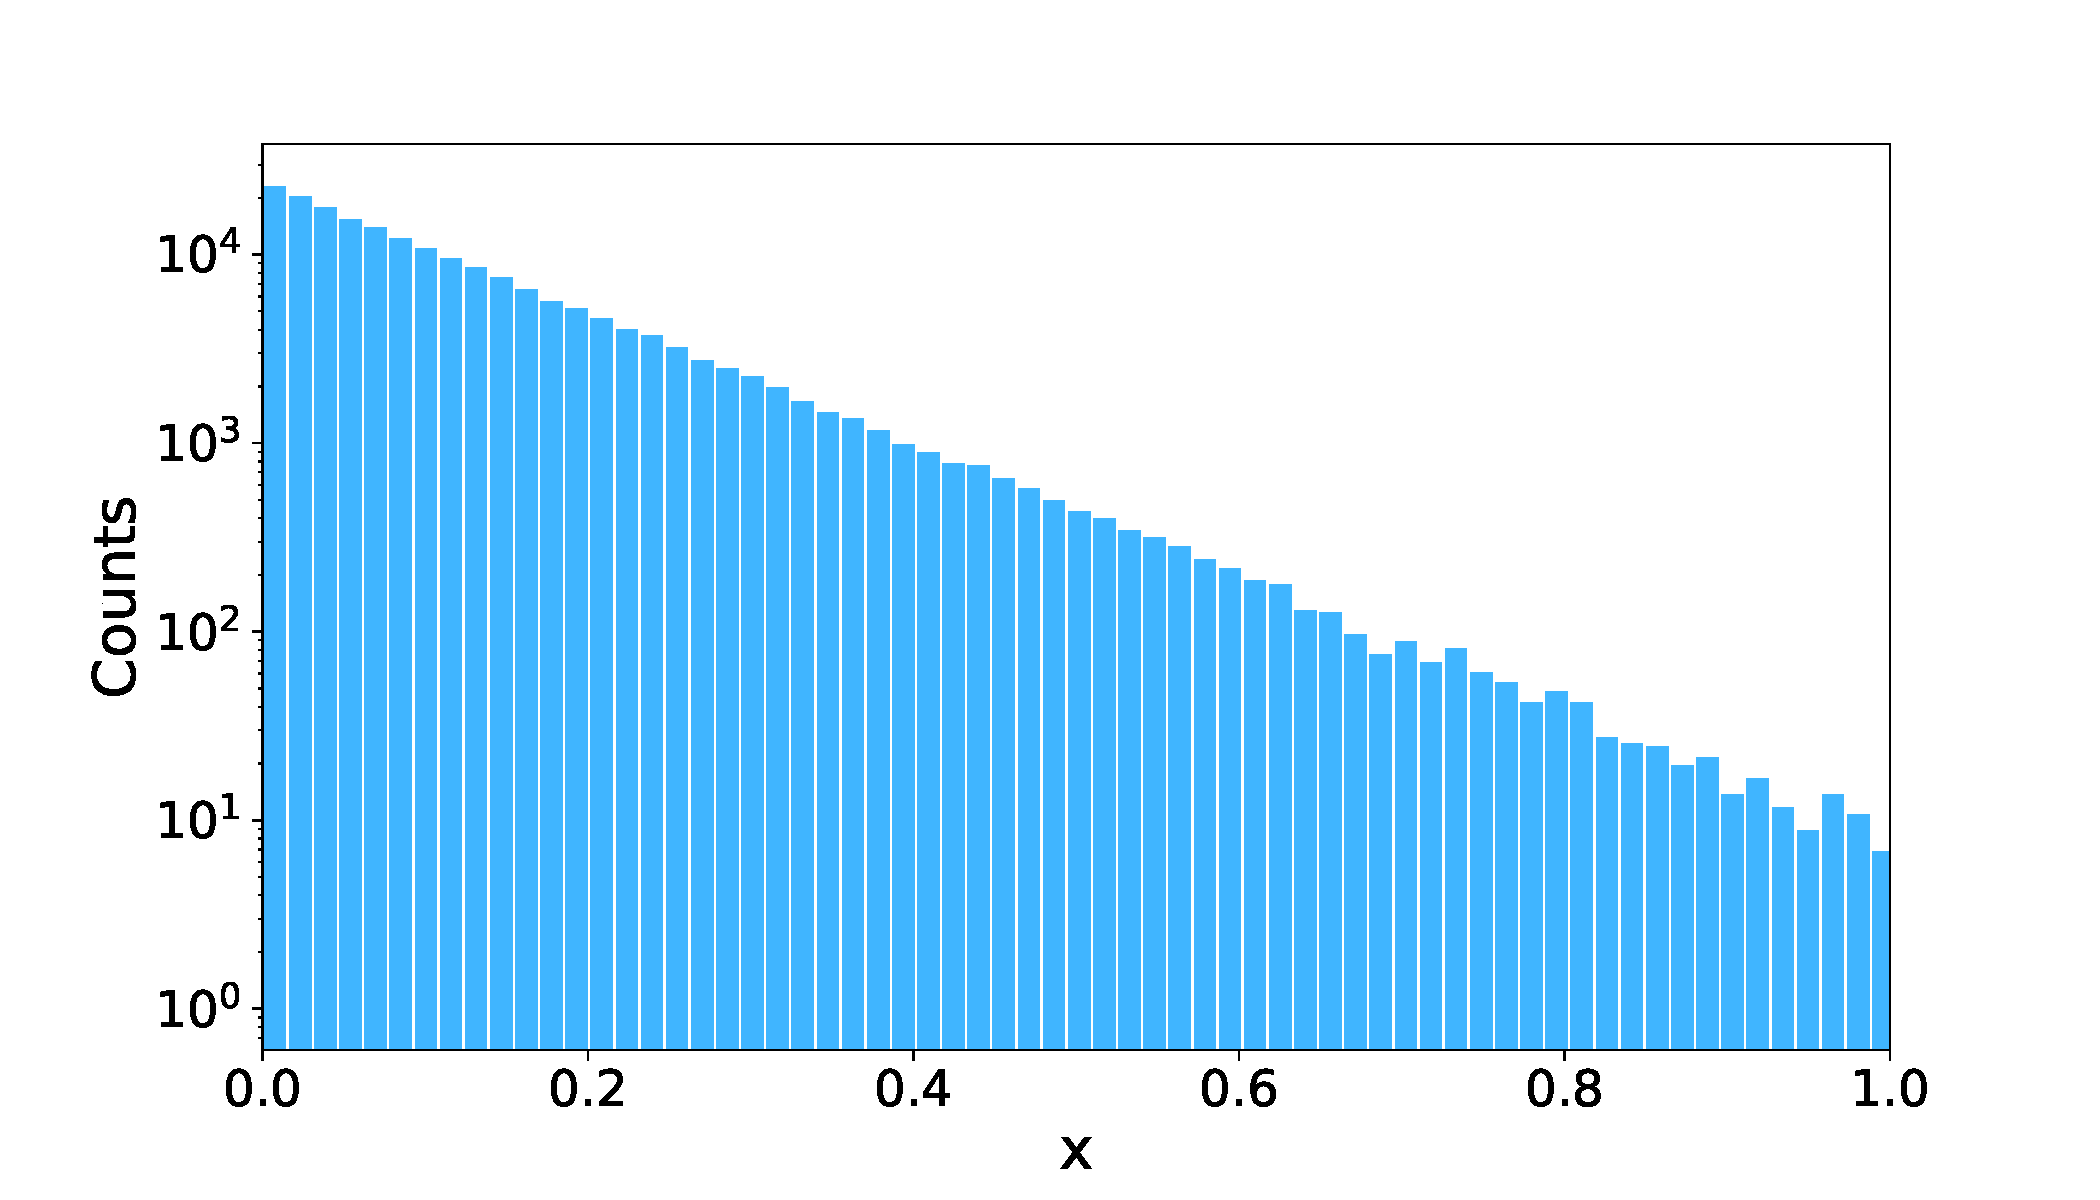
\includegraphics[width=.3\textwidth]{../PLOTS/DISTRIBUTIONS/ref.pdf}};
    \draw[bend left,->, very thick, shorten <=2pt, shorten >=2pt]  (ref) to node [auto] 
    {} (main);


    % LOWER LEFT
    \node(exp)[below left = -1cm and 0cm of main, label={[label distance=-0.4cm]above:\bfseries  data sample $\mathbfcal{D}$}]  
    {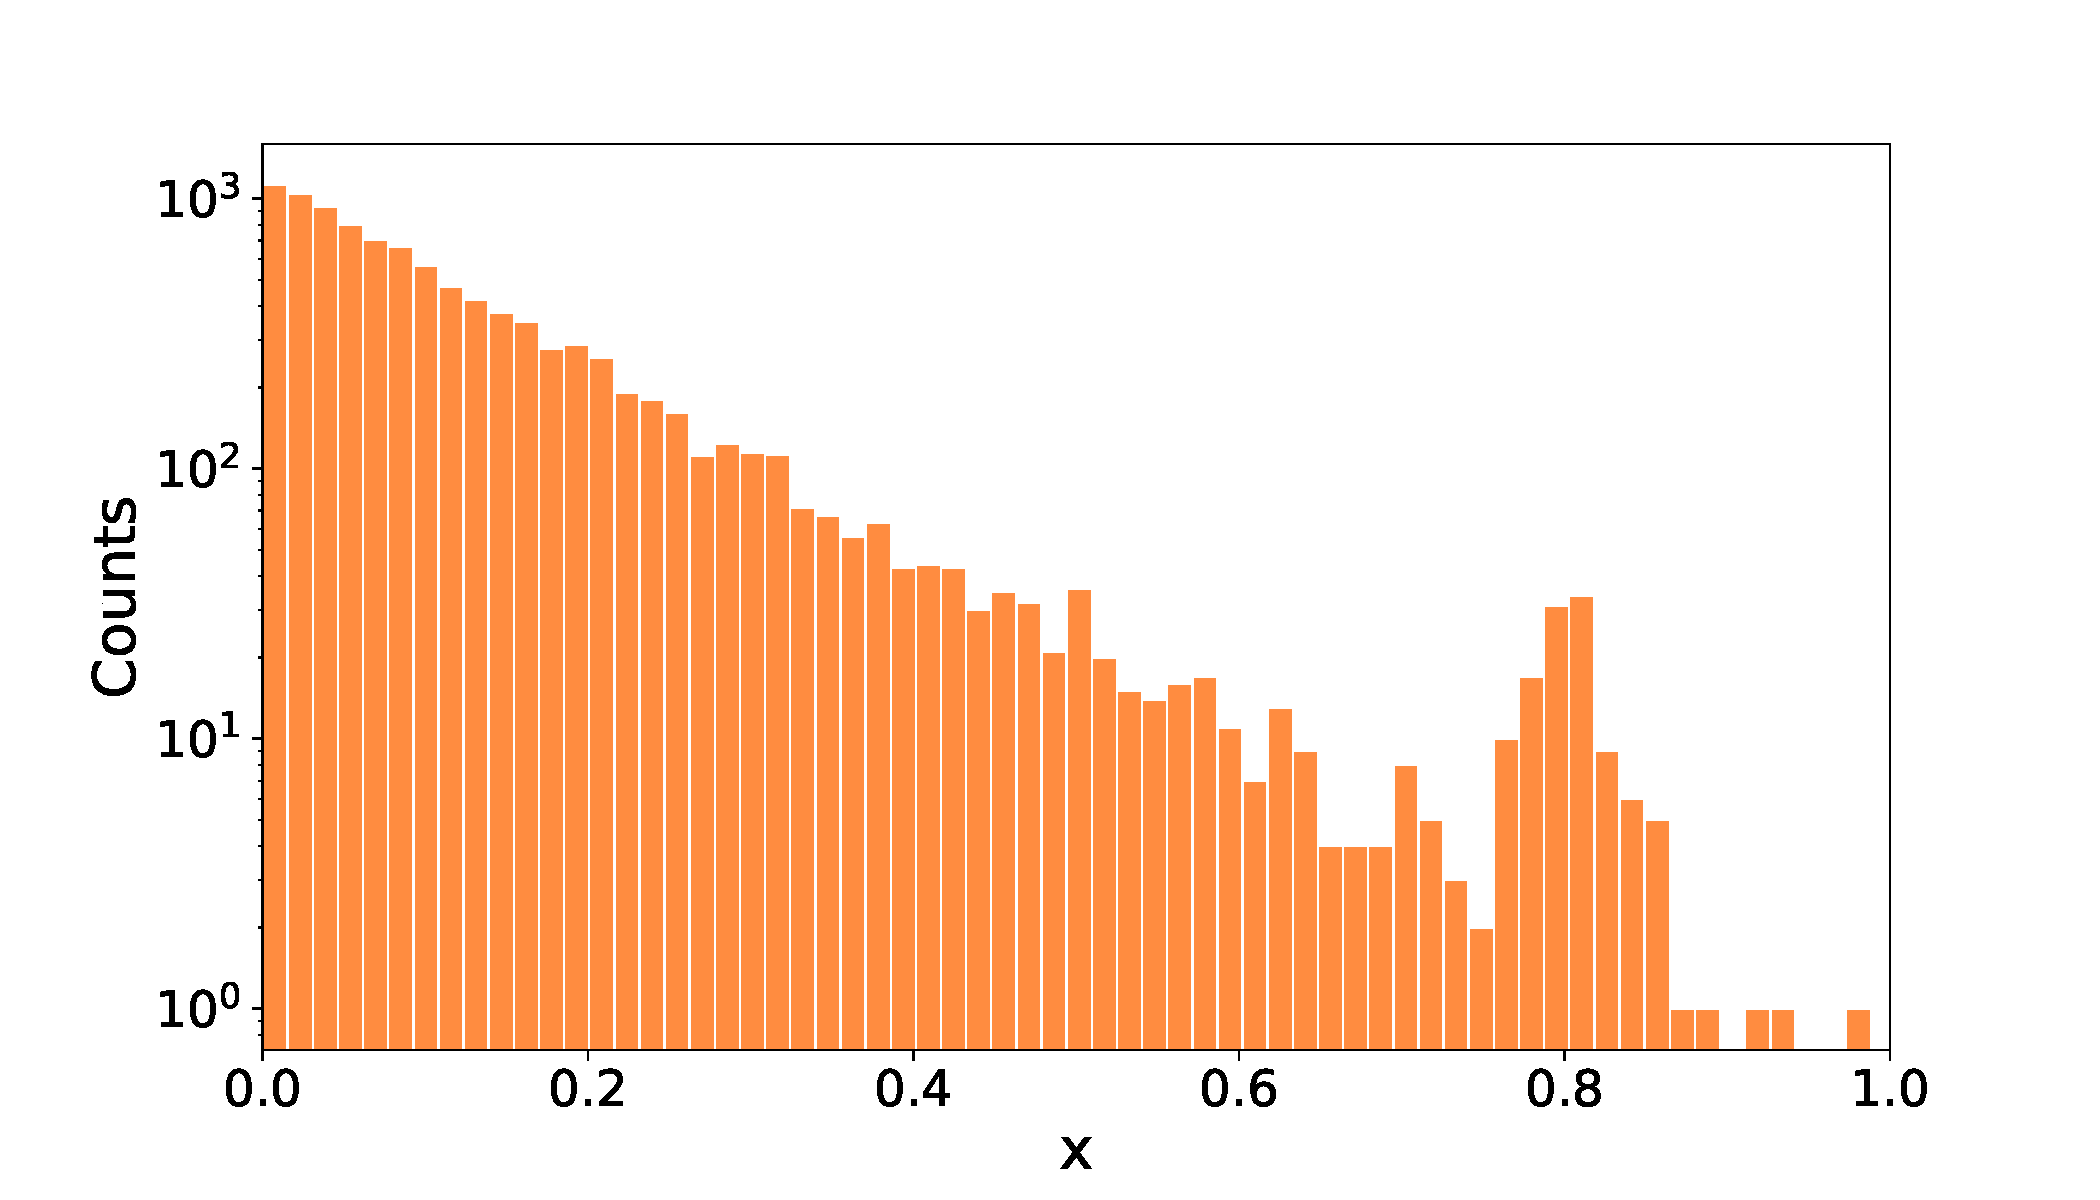
\includegraphics[width=.3\textwidth]{../PLOTS/DISTRIBUTIONS/exp.pdf}};
    \draw[bend right,->, very thick, shorten <=2pt, shorten >=2pt]  (exp) to node [auto] 
    {} (main);

    % UPPER RIGHT
    \node(log)[above right = -1cm and 0cm of main, label={[align=center, label distance=-0.4cm]above:\bfseries  log-ratio distribution \\ 
    $f(x;\,\hat{w})\approx \log\left[\frac{n(x\,|\,\mathbfcal{T})}{n(x\,|\,\mathbfcal{R})}\right]$}] 
    {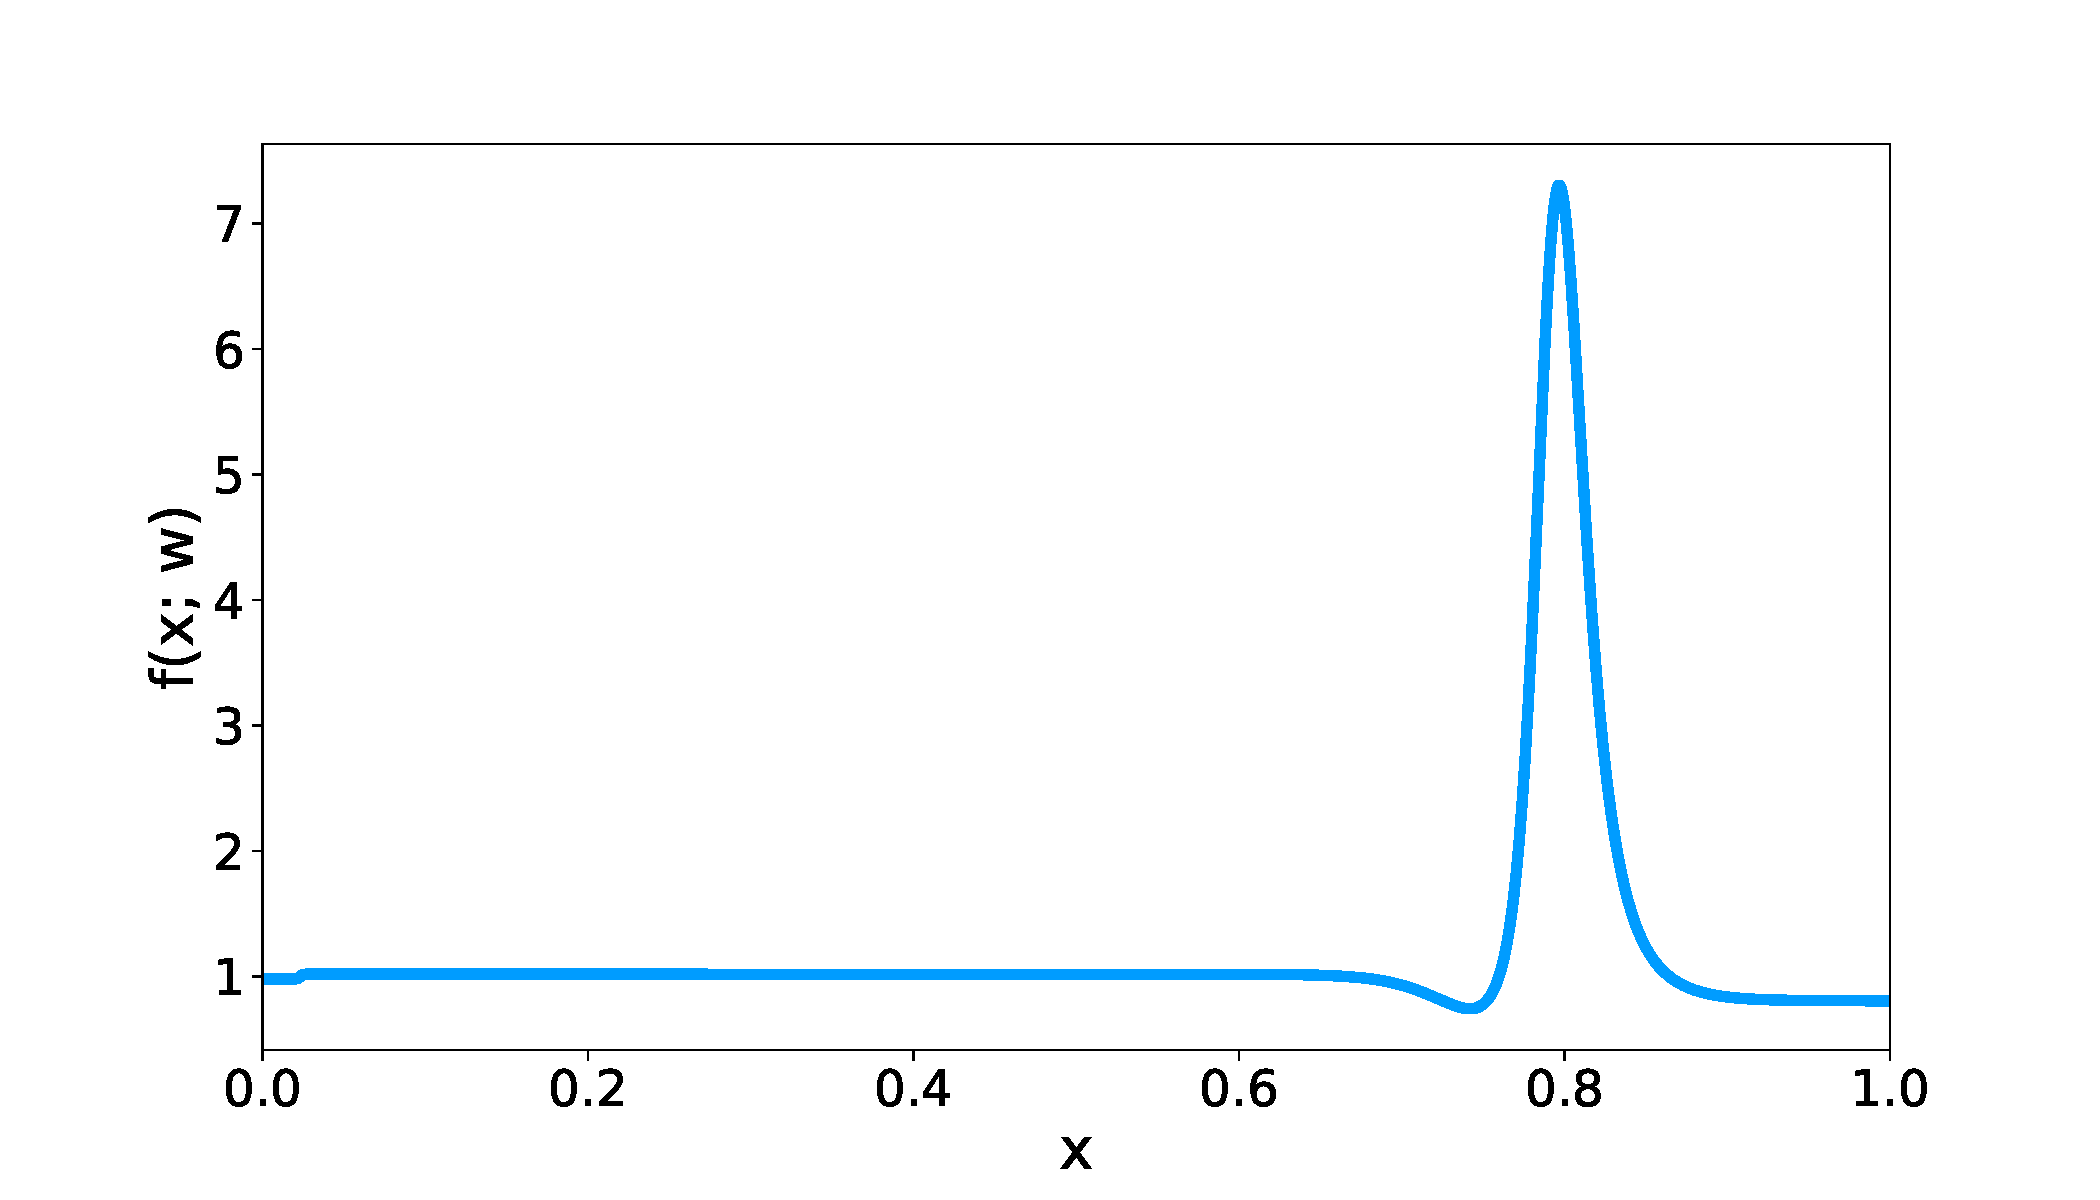
\includegraphics[width=.3\textwidth]{../PLOTS/DISTRIBUTIONS/log_ratio_47.pdf}};
    \draw[bend left,->, very thick, shorten <=2pt, shorten >=2pt]  (main) to node [auto] 
    {} (log);


    % LOWER RIGHT
    \node(t)[below right = -1cm and 0cm of main, label={[align=center, label distance=-0.4cm]above:\bfseries $\boldsymbol{t}$ distribution \\
    $t(\mathbfcal{D})=-2\,\min_w L[f]$}]  
    {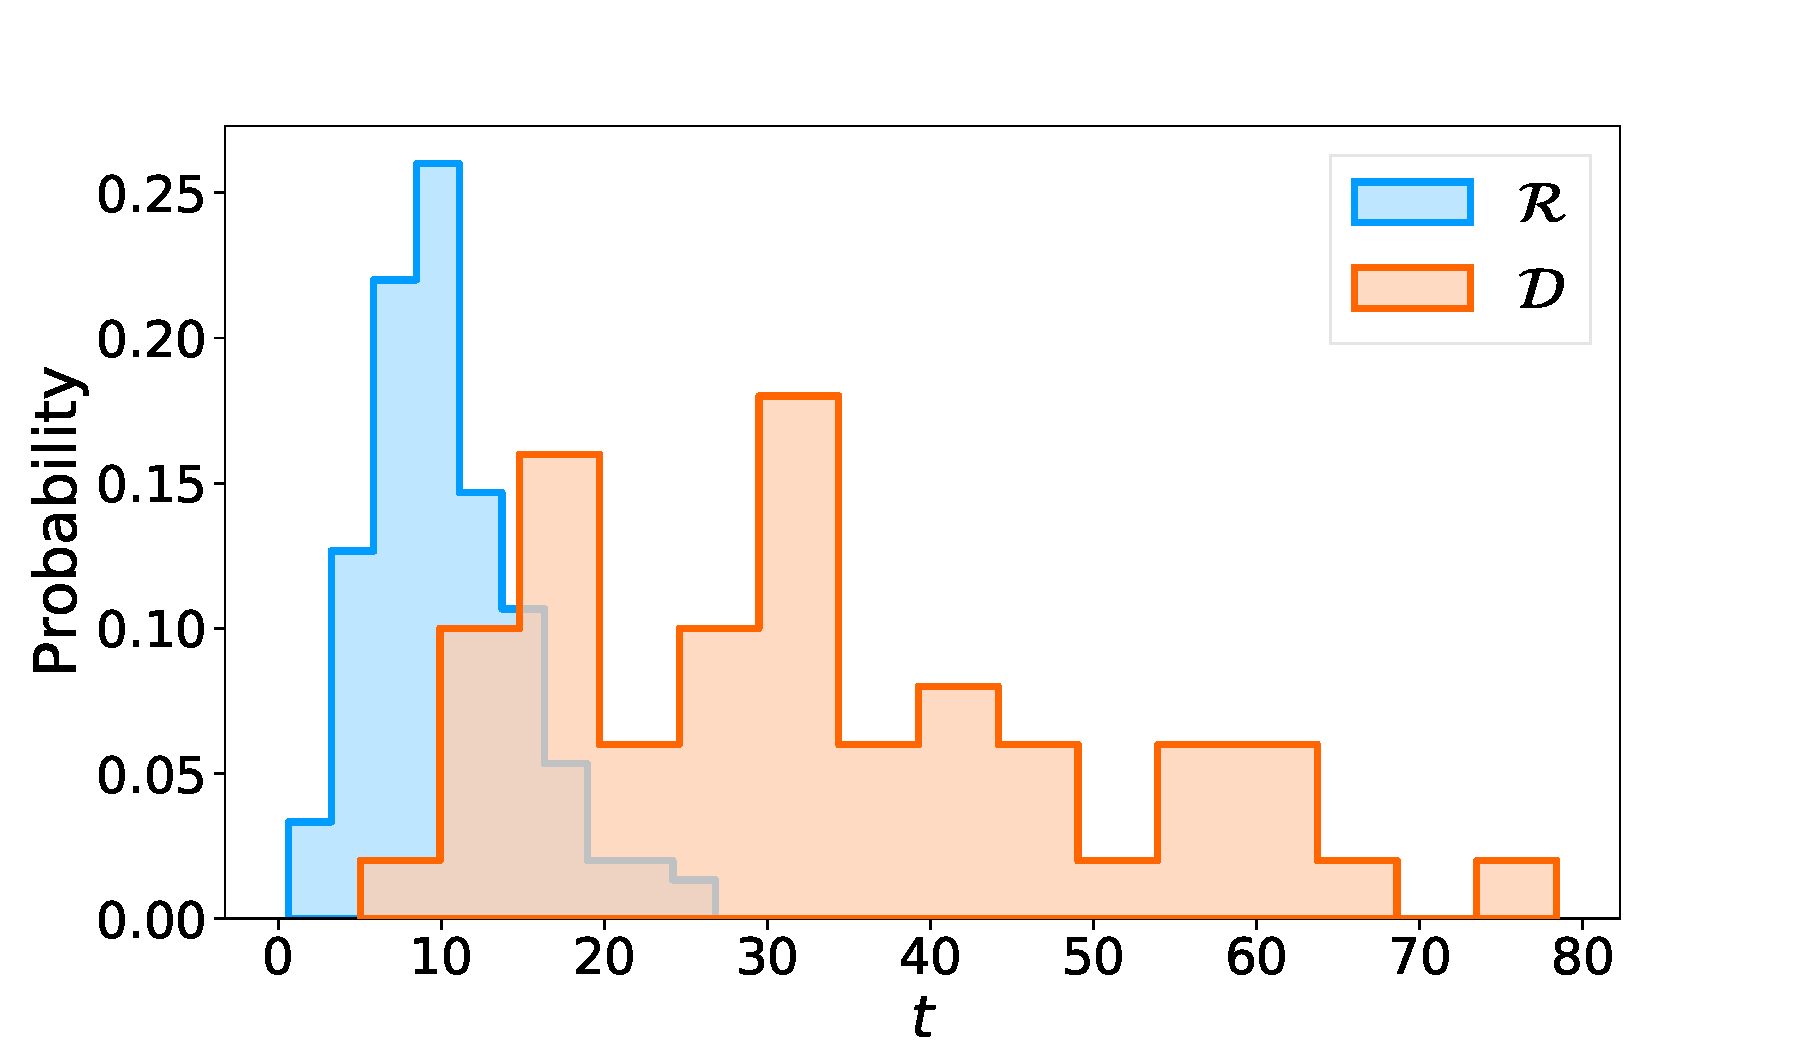
\includegraphics[width=.3\textwidth]{../PLOTS/DISTRIBUTIONS/summary_distribution.pdf}};
    \draw[bend right,->, very thick, shorten <=2pt, shorten >=2pt]  (main) to node [auto] 
    {} (t);

    % INPUT
    \node(in)[above = 1.5cm of ref]{\bfseries INPUT};

    % OUTPUT
    \node(out)[above = 1.5cm of log]{\bfseries OUTPUT};

\end{tikzpicture}}
	\captionof{figure}{Visual representation of the algorithm}
	\label{fig:summary}
\end{figure} 

In order to quantify the probability that a discrepancy is present in $\mathbfcal{D}$, it is necessary to compute the
probability distribution $p(t\,|\,\mathbfcal{R})$ (i.e., the distribution of the test statistic when the reference
hypothesis is true). Hence, repeated training processes are performed on datasets $\mathbfcal{D}_{\mathbfcal{R}}$
sampled from the reference model itself. A convenient result by S. Wilks \cite{wilks} ensures that, as the size of the
data samples, tested using the likelihood ratio, approaches infinity, the distribution of the test statistic under the
null hypothesis asymptotically approaches a $\chi^2$ distribution. The number of degrees of freedom of the distribution
is the difference between the parameter space dimensionality of the two hypotheses. In this case, with neural networks
involved, the number of degrees of freedom is equal to the number of trainable parameters of the network. Thus, if the
training process has adequately worked, the distribution of the test statistic under the null hypothesis (i.e., computed
using $\mathbfcal{D}_{\mathbfcal{R}}$ datasets) should be compatible with the $\chi^2_\nu$ distribution, where $\nu$
stands for the degrees of freedom of the network. Otherwise, more accurate tuning of the network's hyperparameters needs
to be performed\footnote{\textit{Hyperparameters} are the variables that determine the network structure and how the
network is trained. A few examples are the number of hidden layers, the number of neurons in each layer, and the
activation functions.}.

When the NN hyperparameters are tuned correctly, the network is ready to perform on real datasets $\mathbfcal{D}$ coming
from experimental sources. At this point, the procedure described above is replicated, and the test statistic returned by
the network will be called $t_{\text{obs}}$. As previously anticipated, to quantify the probability that a discrepancy
is present in $\mathbfcal{D}$ it is possible to compare $t_{\text{obs}}$ with the $p(t\,|\,\mathbfcal{R})$
distribution. By defining the observed \textit{p}-value as 

\begin{equation}\label{eq:pval}
    p_{\text{obs}}=\int_{t_{\text{obs}}}^{+\infty}p(t\,|\,\mathbfcal{R})\,\text{d}t
\end{equation}

\noindent and its corresponding significance $Z(p)=\Phi^{-1}(1-p)$, where $\Phi^{-1}$ is the quantile of a normal
distribution with $\mu=0$ and $\sigma=1$, a discrepancy in $\mathbfcal{D}$ between $\mathbfcal{R}$ would
manifest itself as a large values of \textit{Z}.  


